% version 1.00	Auteur Michel Cressant

\documentclass[asi, sansVersion]{picInsa}

\usepackage{vocabulaireUnipik}
\usepackage{pdfpages}
\usepackage{graphicx}

\definecolor{gris}{gray}{0.75}
\definecolor{gris2}{gray}{0.85}

\titreGeneral{\FF}
\sousTitreGeneral{Base de Données}
\titreAcronyme{\FFCourt}
\version{}
\referenceVersion{\FFCourt\_Q\_\nomEquipe\_cPHPUnit}
\auteurs{\Pierre{}}
\destinataires{\nomApprobateur{}, \nomTuteurQualite, \nomEquipe}
\resume{Le présent document est la \FF{} à PHPUnit.}
\motsCles{\planQualite{}, PQ, PIC, \nomEquipe{}, \FF}
\natureDerniereModification{Création}
\modeDiffusionControle{}


\begin{document}

	\begin{center}
		\LARGE
		\textsc{
			\FF{}\\
			\No 03 - PHPUnit
		}
	\end{center}
	\vspace{0.5cm}

	\section*{Suivi des modifications}
		\begin{table}[H]
			\centering
			\begin{tabularx}{18cm}{|p{1.7cm}|X|p{4cm}|}
				\hline
				\rowcolor[gray]{0.90} Date & Nature de la modification \\
				\hline
				
				22/02/16 & Création \\
				\hline
			\end{tabularx}
		\end{table}

	\section*{Description}
		\begin{longtable}{|p{0.35\textwidth}|p{0.65\textwidth}|}
			\hline
			\cellcolor{gris2} Intitulé & Formation au framework PHPUnit\\\hline
			\cellcolor{gris2} Date de formation & 29/09/2016 \\\hline
			\cellcolor{gris2} Date d'évaluation à chaud & 29/10/2016 \\\hline
			\cellcolor{gris2} Date d'évaluation à froid & 18/11/2016 \\\hline
			\cellcolor{gris2} Démarche & Afin de maîtriser la création de tests unitaires complexes, il a été nécessaire de former les membres de l'équipe.\\\hline
			\cellcolor{gris2} Évaluation &
				\textbf{Évaluation à chaud} : les membres de l'équipe ont répondu à un exercice noté par \Michel{}. La barre de validation a été fixée à 7 / 10.\newline
				\textbf{Évaluation à froid} : mise en œuvre des compétences acquises pour la réalisation du lot n°2.\\\hline
			\cellcolor{gris2} Évaluateurs & \Michel{}\\\hline
			\cellcolor{gris2} Membres évalués & \Melissa{}, \Matthieu{}, \Mathieu{}, \Florian{}, \Kafui{}\\\hline
			\cellcolor{gris2} Membres reçus & N/A \\\hline
			\cellcolor{gris2} Supports & Les membres ont étudié les documents aux adresses : \begin{itemize}
			\item La documentation officielle de Symfony (Partie "The PHPUnit Testing Framework") : \url{http://symfony.com/doc/current/book/testing.html}
			\item La documentation officielle de Symfony (Partie "How to Test Doctrine Repositories") : \url{http://symfony.com/doc/current/cookbook/testing/doctrine.html} 
			\item L'utilisation de doctrine (Partie "Functionnal Testing") :
\url{http://symfony2-document.readthedocs.org/en/latest/cookbook/testing/doctrine.html}
		\end{itemize}
			 \\\hline
			\cellcolor{gris2} Terminée & Non \\\hline
		\end{longtable}

	\newpage
	\section*{Évaluation à chaud}
		\subsection*{Exercices}
		Pour cette évaluation, vous ferez les exercices suivants : 
		\\
		
	%	\textbf{Exercice 1 :}\\
	%	Réaliser le diagramme d'activité suivant : 
	%	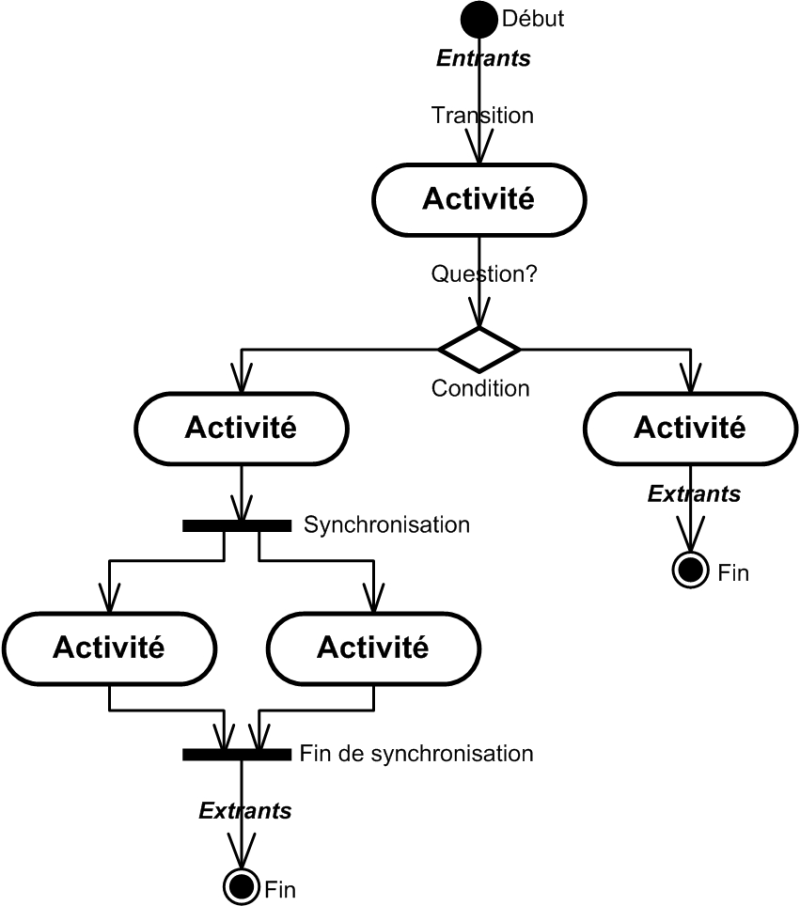
\includegraphics[scale=0.6]{diagrammeDActivite.png}
		\textbf{Exercice 1 :}\\
		Ecrire la classe HelloUnicefTest contenant les méthodes suivantes :
		\begin{itemize}
			\item testLinkFromIndex() qui test la redirection vers la page 'Hello Unicef !' en cliquant sur l'index;
			\item testLinkFromNavbar() qui test la redirection vers la page 'Hello Unicef !' en cliquant sur la barre de navigation;
			\item tesHelloUnicef() qui test que la page située à l'url /unicef/hello posséde les mots 'Hello Unicef !'.
		\end{itemize}
		
		\textbf{Exercice 2 :}\\
		Ecrire la classe VolunteerTest contenant le test suivant : 
		\begin{itemize}
			\item testVolunteer() qui créée un nouveau volontaire, le stock en BD, le récupère et vérifie que ses informations correspondent à celles données lors de la création.
		\end{itemize}
		
			\vspace{8px}
			
		\subsection*{Résultats}
			\begin{longtable}{|p{0.5\textwidth}|p{0.5\textwidth}|}
				\hline
					\rowcolor[gray]{0.90} Nom & Note (/10) \\
				
				\hline
					\Mathieu & N/A \\
				\hline
					\Matthieu & N/A \\
				\hline
					\Kafui & N/A \\
				\hline
					\Melissa & N/A \\
				\hline
					\Florian & N/A \\
				\hline
			
			\end{longtable}
			
	\newpage
	\section*{Évaluation à froid}
		L'évaluation à froid correspond à la réalisation des tests unitaires sur les lots 3 et 4.

\end{document}
